\section{Theorie}
\subsection{Magnetismus}
Magnetismus ist eine Eigenschaft von (jedem) Stoff und ist eine der vier Grundkräfte der Physik (wie z.B. auch Gravitation). Hierbei kann man den Magnetismus in die drei wichtigsten Formen unterteilen:
\begin{itemize}
\item Diamagnetismus
\item Paramagnetismus
\item Ferromagnetismus
\end{itemize}
\textbf{Diamagnetische Stoffe} haben keine permanenten Dipole, innerhalb von Magnetfeldern entstehen induzierte Dipole, deren Ausrichtung dem äußeren Magnetfeld entgegengerichtet sind.
\begin{align*}
\vec{M}=\chi \vec{H}\text{,}
\end{align*}
wobei $\chi$ (Suszeptibilität) negativ ist.\\
Ein Beispiel für einen diamagnetischen Stoff ist Kohlenstoff. \\
\textbf{Paramagnetische Stoffe} haben permanente magnetische Dipole, welche aber ohne äußeres Magnetfeld nicht ausgerichtet und damit insgesamt die Summe null haben:
\begin{align*}
\vec{M}&=\frac{1}{V}\sum_m \vec{p}_m\text{.}
\end{align*}
In einem äußeren Magnetfeld richten sich die Dipole im Stoff teilweise aus.\\
Ein Beispiel hierfür sind Alkalimetalle.

\subsection{Ferromagnetismus}
Der dritte (Haupt-)Fall von Magnetismus ist der Ferromagnetismus. Hierbei ist die Suszeptibilität $\chi$ sehr groß und die Magnetisierung sehr viel größer als bei Paramagneten. In einem äußeren Magnetfeld ist die Magnetisierung keine eindeutige Funktion. Trägt man für einen (davor) vollkommen entmagnetisierten Stoff die Magnetisierung gegen das Magnetfeld auf, bekommt man eine sogenannte Hysteresekurve (siehe Abb. (\ref{hysterese})). Die Magnetisierung wächst mit dem Magnetfeld bis eine Sättigung erreicht wird. Beim abschwächen des Magnetfeldes sinkt die Magnetisierung nicht auf der gleichen Kurve.
\begin{figure}[!htbp]
\centering
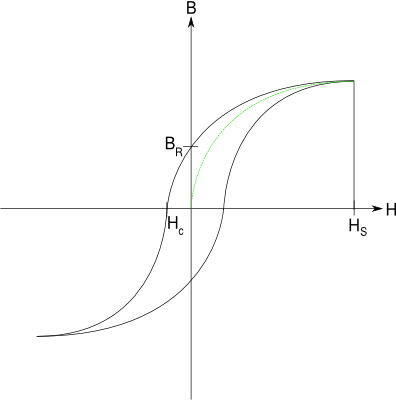
\includegraphics[width=5cm]{hysterese.png}
\caption{Hysteresekurve der Magnetisierung in Abhängigkeit vom Magnetfeld} \label{hysterese}
\end{figure}
Das klassische Beispiel für einen ferromagnetischen Stoff ist Eisen.\\
Bei Ferromagneten lassen sich noch weitere Merkmale beobachten. Zum Beispiel verschwindet der Ferromagnetismus im Stoff, wenn dieser über eine Grenztemperatur $T_C$, auch \textbf{Curie-Temperatur} genannt, erhitzt wird. Der Paramagnetismus hingegen verschwindet aber nicht. Desweiteren lassen sich Ferromagneten in sog. \textbf{Weisssche Bezirke} unterteilen. Diese Bezirke sind etwa $10^{-5}$ bis $10^{-3}$ Meter linear ausgedehnt. Innerhalb solcher Bezirke sind die Dipole gleichgerichtet. Die Grenzen zwischen solchen Bezirken heißen \textbf{Bloch-Wände}. Legt man ein Magnetfeld an, verschieben sich diese Bloch-Wände, sodass die Gebiete mit gleicher Ausrichtung wie das äußere Feld größer werden. Wächst das Feld immer weiter polen sich die Weiss-Bezirke schlagartig um. Dieser Effekt heißt \textbf{Barkhausen-Sprung} und kann mithilfe einer Spule hörbar gemacht werden.
\begin{figure}[!htbp]
\subfigure[Weissscher Bezirk]{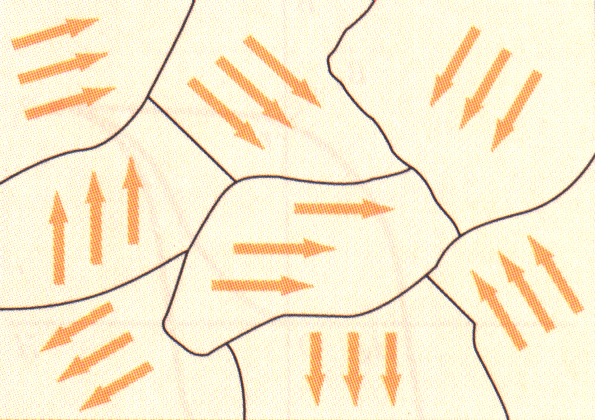
\includegraphics[width=0.49\textwidth]{weiss.png}}\hfill
\subfigure[Weissscher Bezirk in abh. von der Curie-Temperatur]{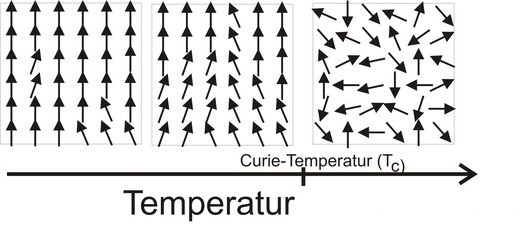
\includegraphics[width=0.49\textwidth]{curie.png}}
%http://web.physik.rwth-aachen.de/~hebbeker/lectures/ph2_02/tipl278.gif (1)
%http://media.supermagnete.de/terms/medium/pu59.jpg (2)
 \label{weiss}
\end{figure}

\subsection{Ausgerichtete Elektronen pro Atomkern}
Mithilfe der Sättigungsmagnetisierung $B_{Sätt}$ lässt sich die Anzahl der pro Eisenkern ausgerichteten Elektronen. Die Magnetisierung $M=\frac{an\mu_\beta}{V}$ ($n$ Atome mit $a$ ausgelenkten Elektronen mit dem magn. Moment $\mu_\beta$ (Bohrsches Magneton)) ist die Anzahl der magnetischen Dipole pro Volumen $V$.\\
Mithilfe von $M=\chi H=\frac{B_{Sätt}}{\mu_0}$ ergibt sich die Formel für die Anzahl der ausgerichteten Elektronen (pro Atomkern):
\begin{align}
a=\frac{M_{N_A} M}{N_A\mu_B\rho}\text, \label{aepa}
\end{align}
wobei $M_{N_A}$ die Molmasse, $N_A$ die Avogadrokonstante und $\rho$ die Dichte des Stoffes ist.